\documentclass{ximera}

%% You can put user macros here
%% However, you cannot make new environments

\listfiles

\graphicspath{{./}{firstExample/}{secondExample/}}

\usepackage{tikz}
\usepackage{tkz-euclide}
\usepackage{tikz-3dplot}
\usepackage{tikz-cd}
\usetikzlibrary{shapes.geometric}
\usetikzlibrary{arrows}
\usetikzlibrary{decorations.pathmorphing,patterns}
\usetkzobj{all}
\pgfplotsset{compat=1.13} % prevents compile error.

\renewcommand{\vec}[1]{\mathbf{#1}}
\newcommand{\RR}{\mathbb{R}}
\newcommand{\dfn}{\textit}
\newcommand{\dotp}{\cdot}
\newcommand{\id}{\text{id}}
\newcommand\norm[1]{\left\lVert#1\right\rVert}
 
\newtheorem{general}{Generalization}
\newtheorem{initprob}{Exploration Problem}

\tikzstyle geometryDiagrams=[ultra thick,color=blue!50!black]

\usepackage{mathtools}

\title{4.1 Exponential Growth and Decay}%\label{Module 7-ADEF}

\begin{document}

\begin{abstract}
We solve a separable differential equation and describe a few of its many applications.
\end{abstract}

\maketitle

\section*{Exponential Growth and Decay}

Since the applications in this section deal with functions of time, we'll
 denote the independent variable by $t$. If $Q$ is a function of
$t$, $Q'$ will denote the derivative of $Q$ with respect to $t$;
thus,
$$
Q'=\frac{dQ}{dt}.
$$

\subsection*{Exponential Growth and Decay}

One of the most common mathematical models for a physical process is
the \textit{exponential model}, where it's assumed that the rate
of change of a quantity $Q$ is proportional to $Q$; thus
\begin{equation} \label{eq:4.1.1}
Q'=aQ,
\end{equation}
 where $a$ is the constant of proportionality.

The general solution of
\eqref{eq:4.1.1} is
$$
Q=ce^{at}
$$
 and the solution of the initial value problem
$$
Q'=aQ, \quad Q(t_0)=Q_0
$$
 is
\begin{equation} \label{eq:4.1.2}
Q=Q_0e^{a(t-t_0)}.
\end{equation}
Since the solutions of $Q'=aQ$ are exponential functions, we say that
a
quantity $Q$ that satisfies this equation \textit{grows exponentially} if
$a > 0$, or \textit{decays exponentially} if $a < 0$ (see figure below).

\begin{image}
 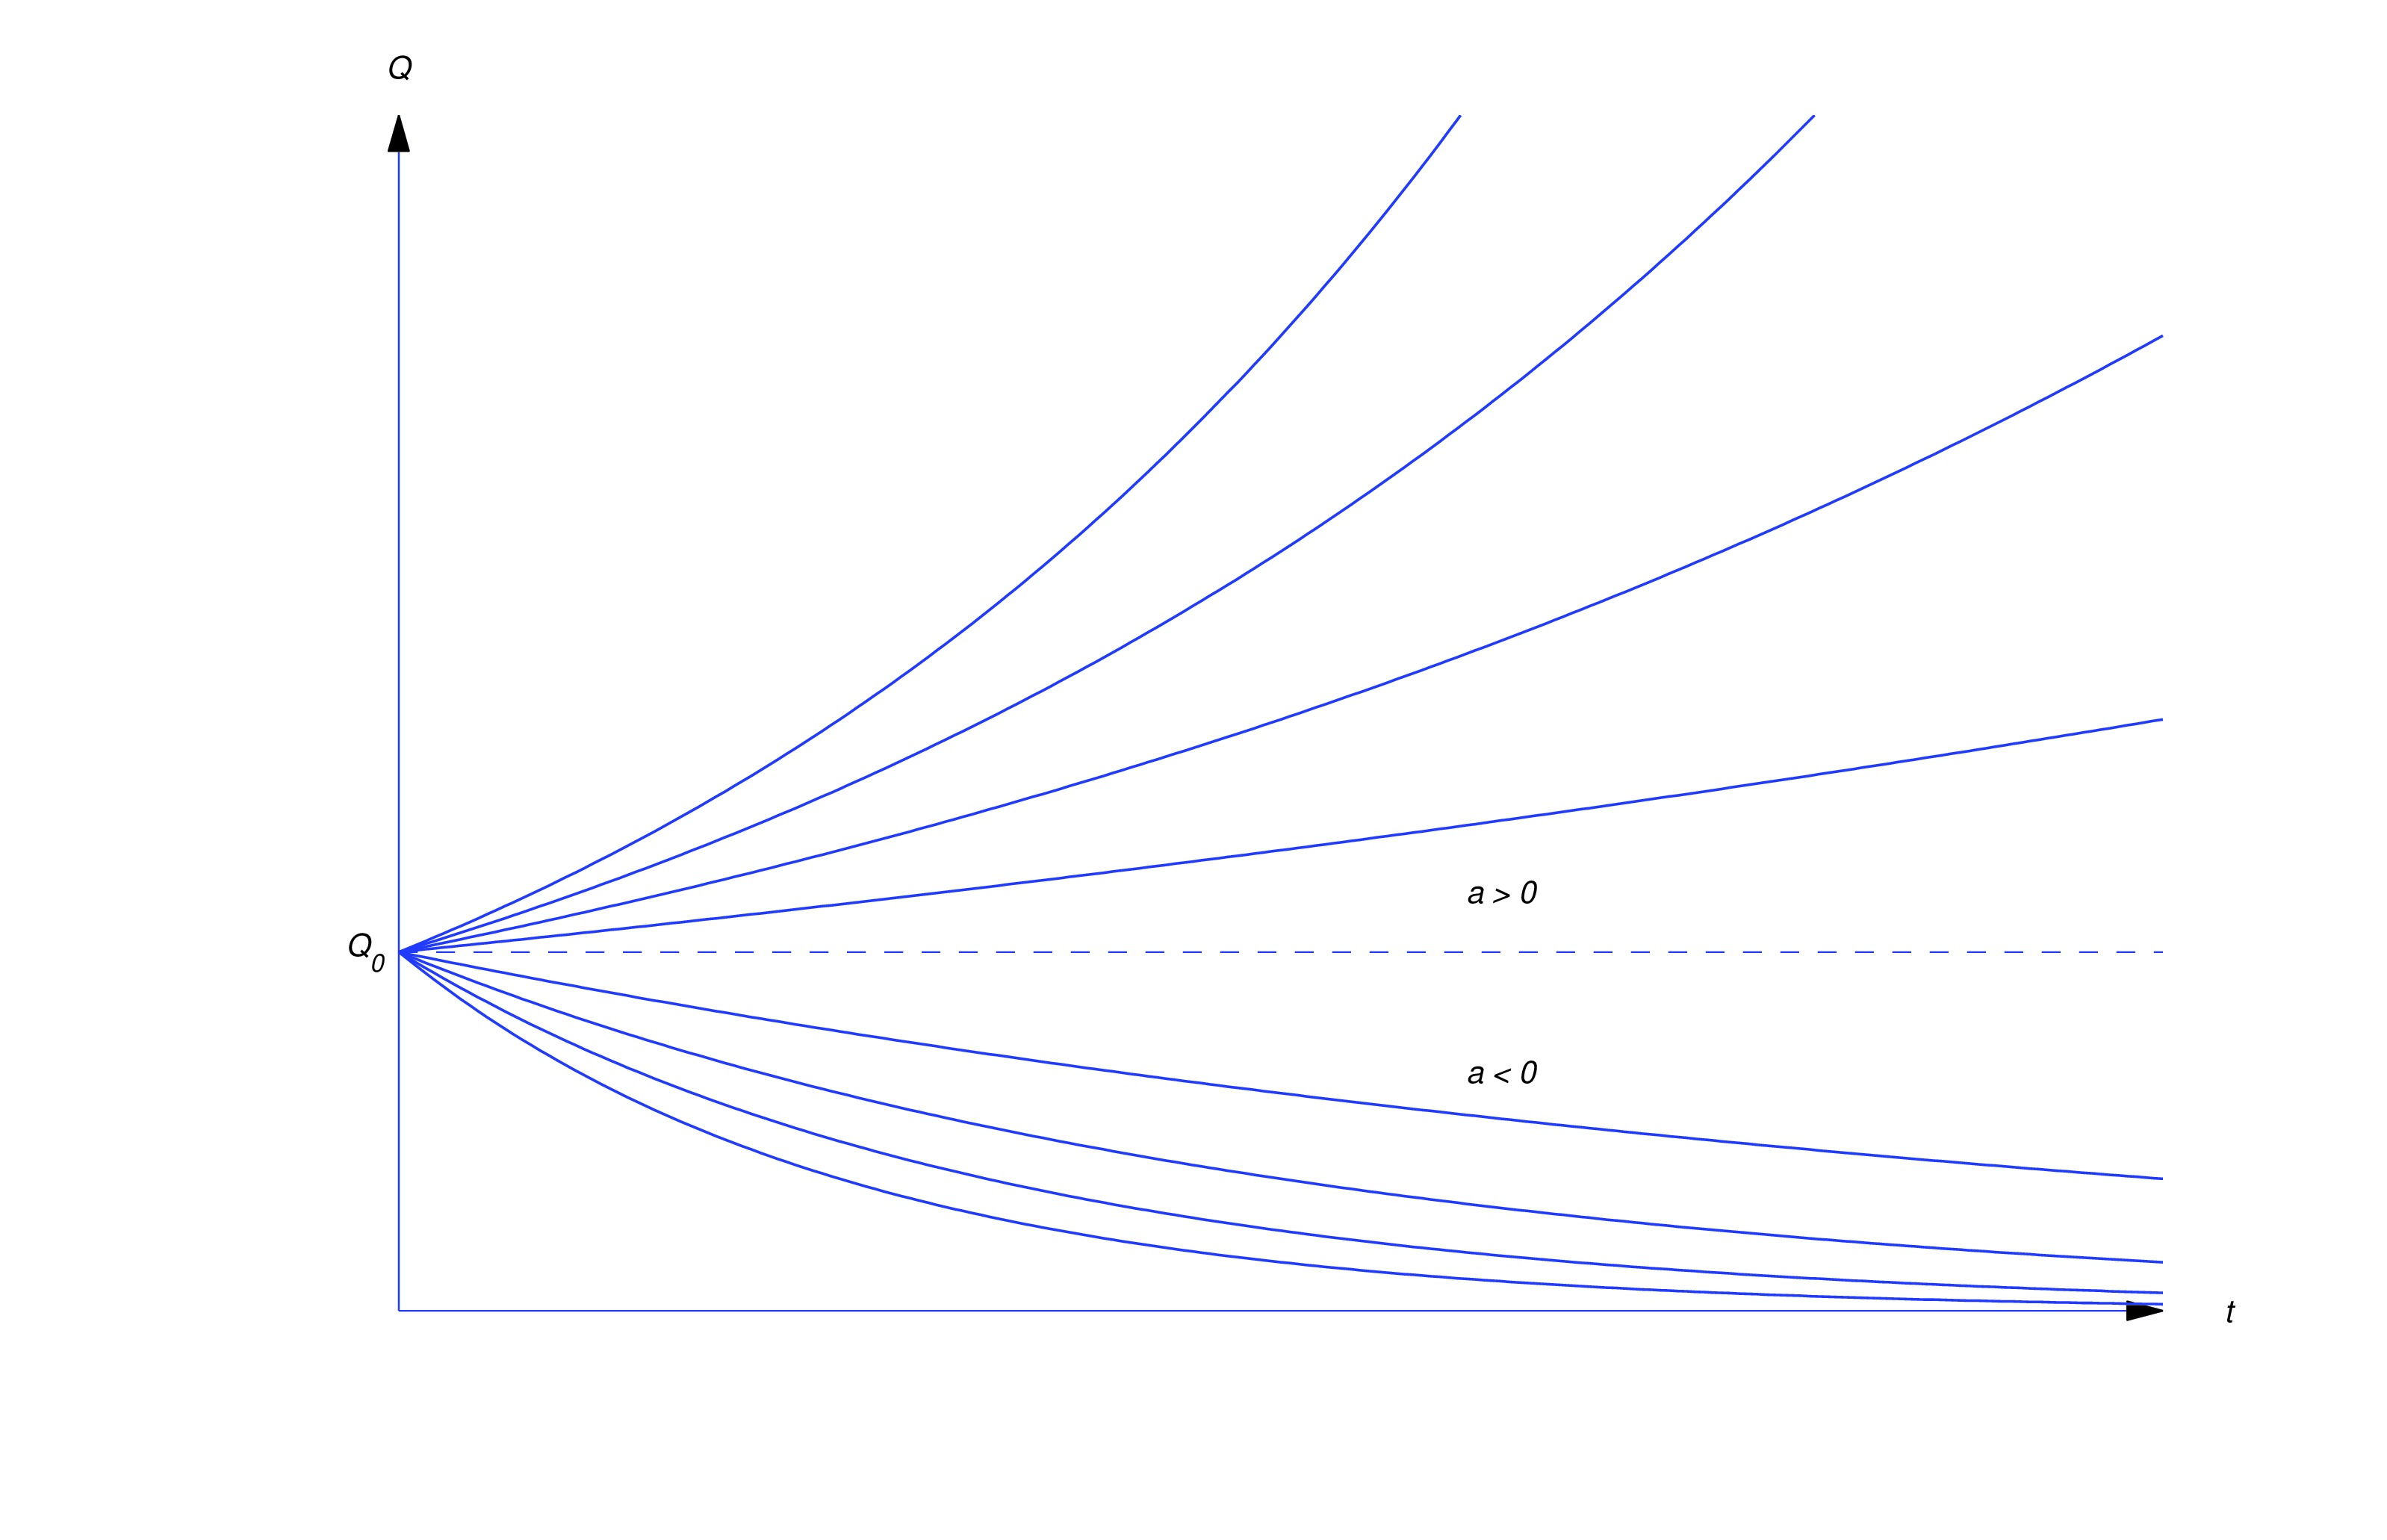
\includegraphics[height=1.5in]{fig040101.jpg} 
\end{image}

%  (Figure~\ref{figure:4.1.1}).

% \begin{figure}[tbp]
%   \centering
%   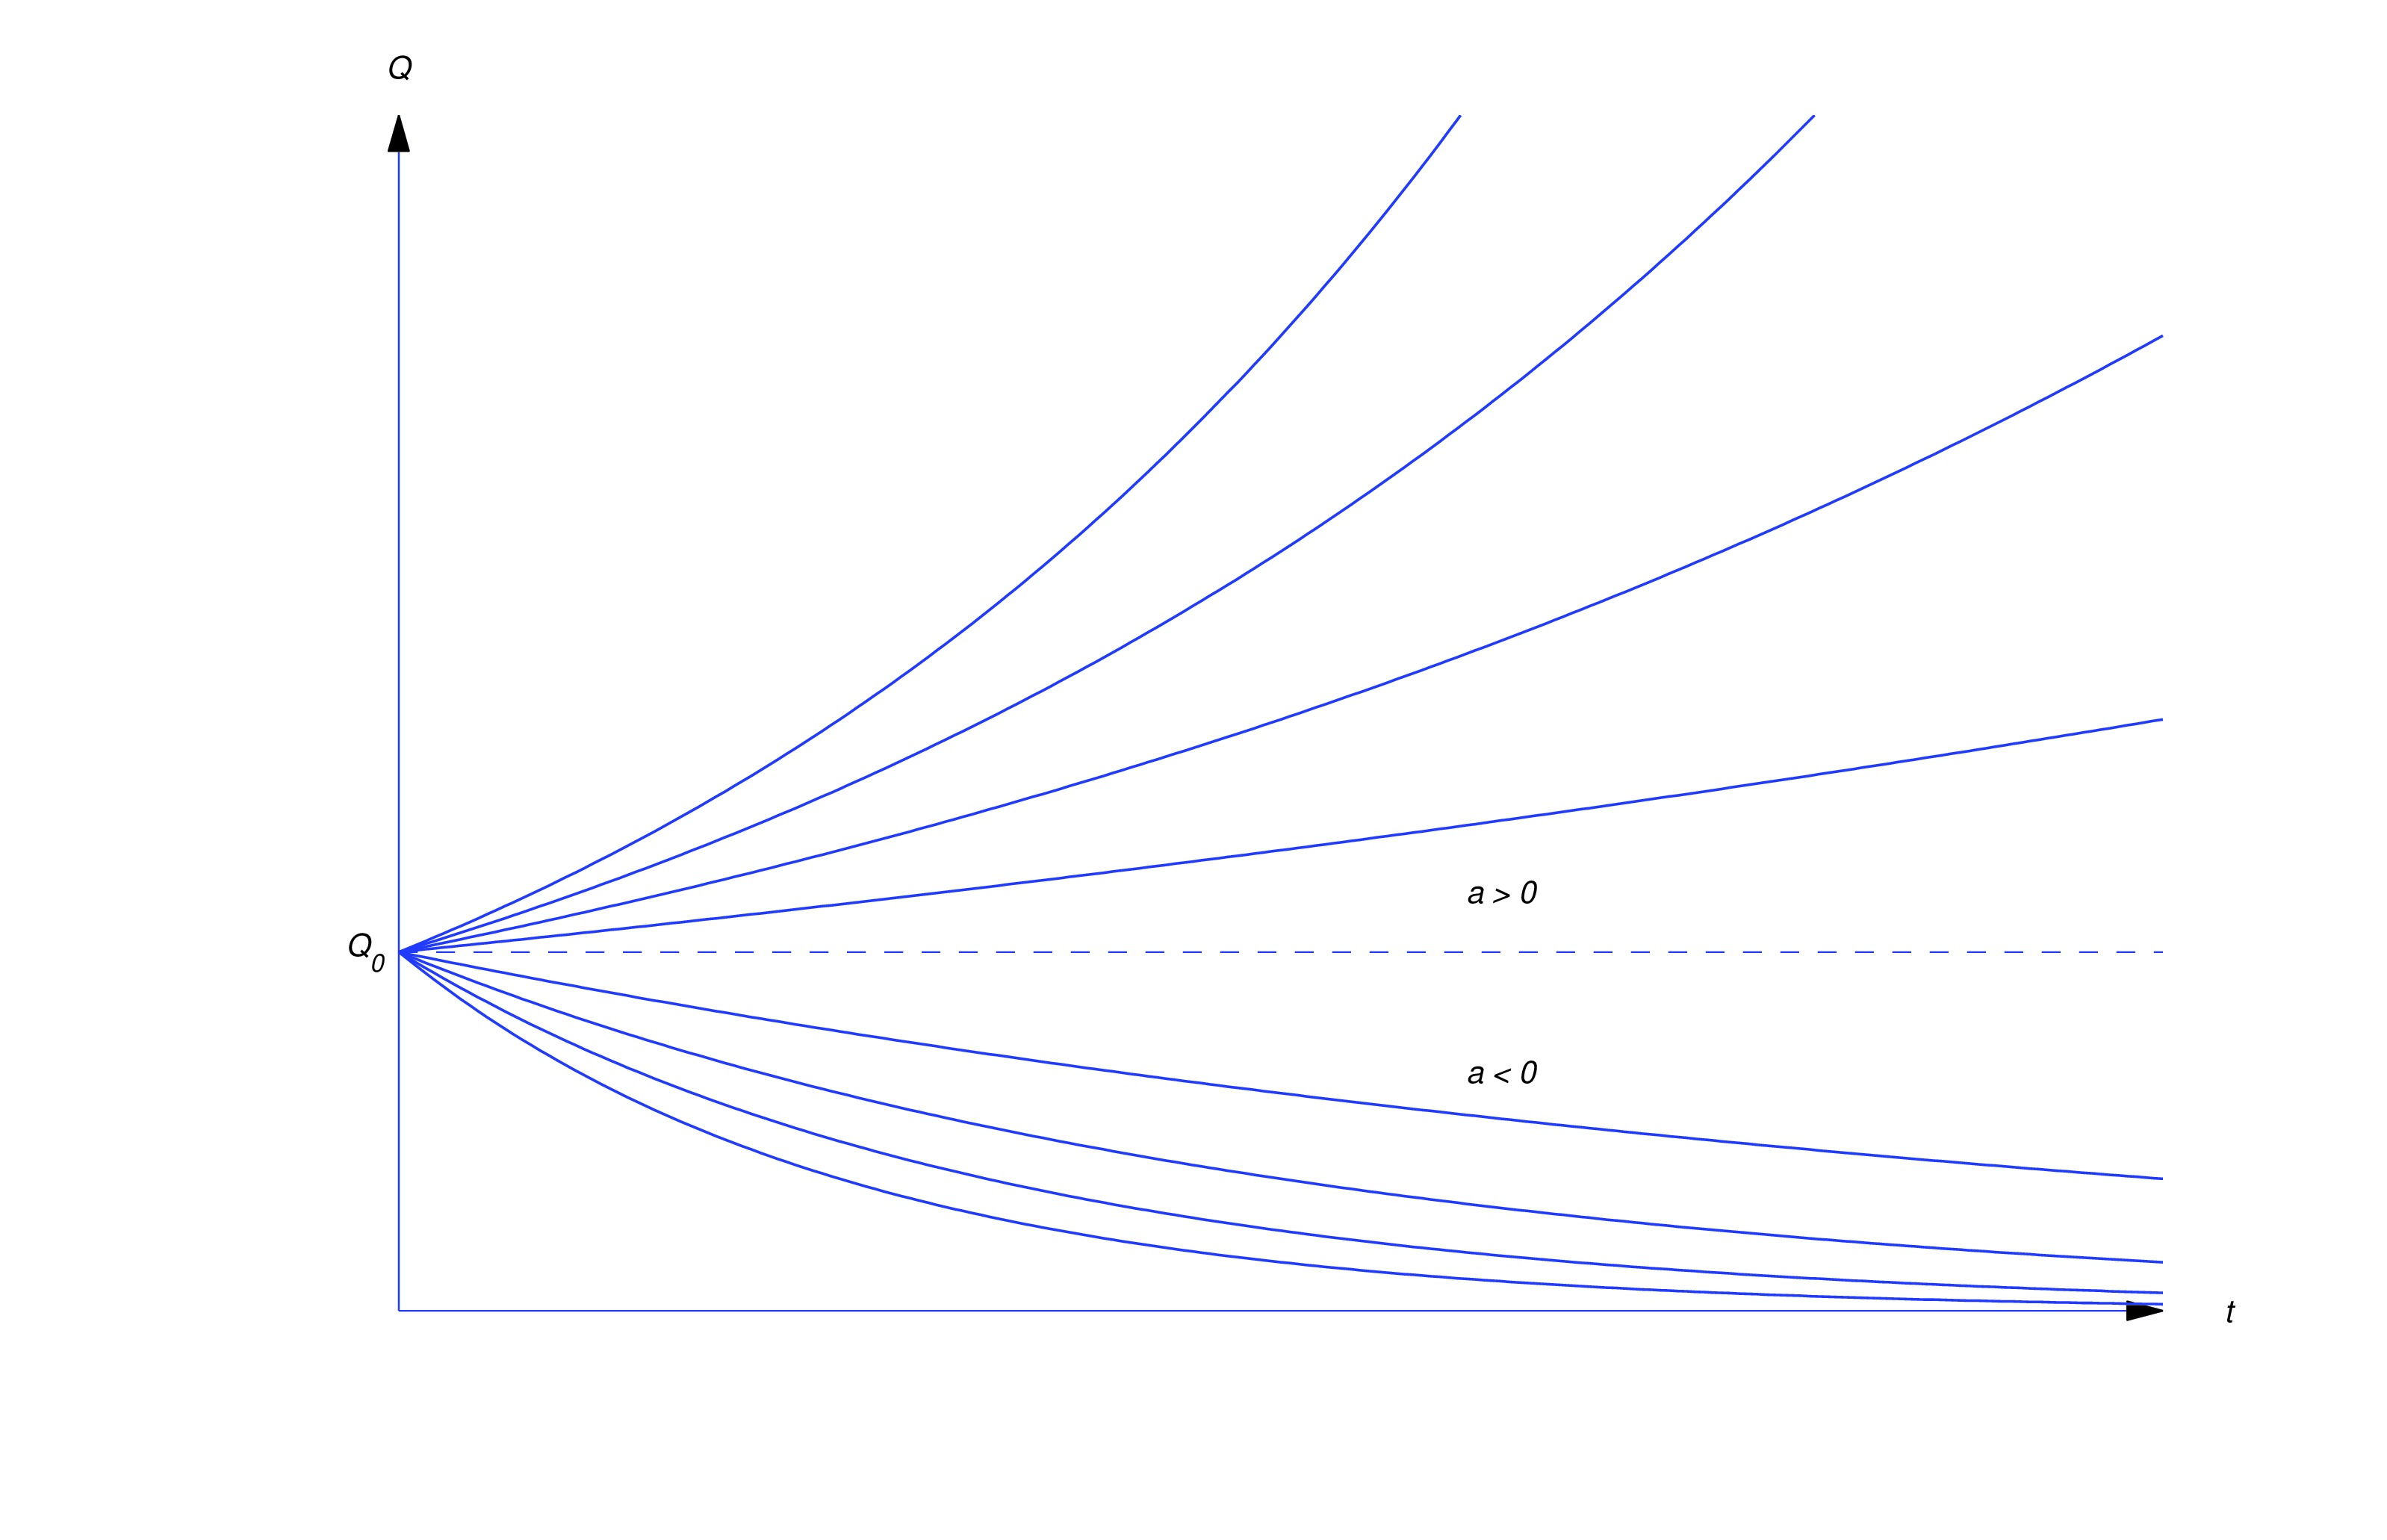
\includegraphics[bb=-78 148 689 643,width=5.67in,height=3.66in,keepaspectratio]{fig040101}
% \color{blue}
% \caption{\label{figure:4.1.1} Exponential growth  and decay}
%   \label{figure4.1.1}
% \end{figure}


\subsection*{Radioactive Decay}

Experimental evidence shows that radioactive material decays at a rate
proportional to the mass of the material present. According to this
model the mass $Q(t)$ of a radioactive material present at time $t$
satisfies \eqref{eq:4.1.1}, where $a$ is a negative constant whose value
for any given material must be determined by experimental observation.
For simplicity, we'll replace the negative constant $a$ by
$-k$, where
$k$ is a positive number that we'll call the \textit{decay constant}
of the material. Thus, \eqref{eq:4.1.1} becomes
$$
Q'=-kQ.
$$
If the mass of the material present
at $t=t_0$ is $Q_0$,  the mass present at time $t$ is
 the solution of
$$
Q'=-kQ,\quad  Q(t_0)=Q_0.
$$
From \eqref{eq:4.1.2}  with $a=-k$, the solution of this initial value
problem is
\begin{equation} \label{eq:4.1.3}
Q=Q_0e^{-k(t-t_0)}.
\end{equation}

The \textit{half--life} $\tau$ of a radioactive material is defined to be
the time required for half of its mass to decay; that is, if
$Q(t_0)=Q_0$, then \begin{equation} \label{eq:4.1.4} Q(\tau+t_0)=\frac{Q_0}{2}.
\end{equation}
 From \eqref{eq:4.1.3} with $t=\tau+t_0$, \eqref{eq:4.1.4} is equivalent to
$$
Q_0e^{-k\tau}=\frac{Q_0}{2},
$$
 so
$$
e^{-k\tau}=\frac{1}{2}.
$$
 Taking logarithms  yields
$$
-k\tau=\ln\frac{1}{2}=-\ln2,
$$
 so the half-life is
\begin{equation} \label{eq:4.1.5}
\tau=\frac{1}{k}\ln2.
\end{equation}
(see figure below).
%(Figure \ref{figure:4.1.2}). 
The half-life is independent of $t_0$ and
$Q_0$, since it's determined by the properties of material, not by
the amount of the material present at any particular time.

\begin{image}
 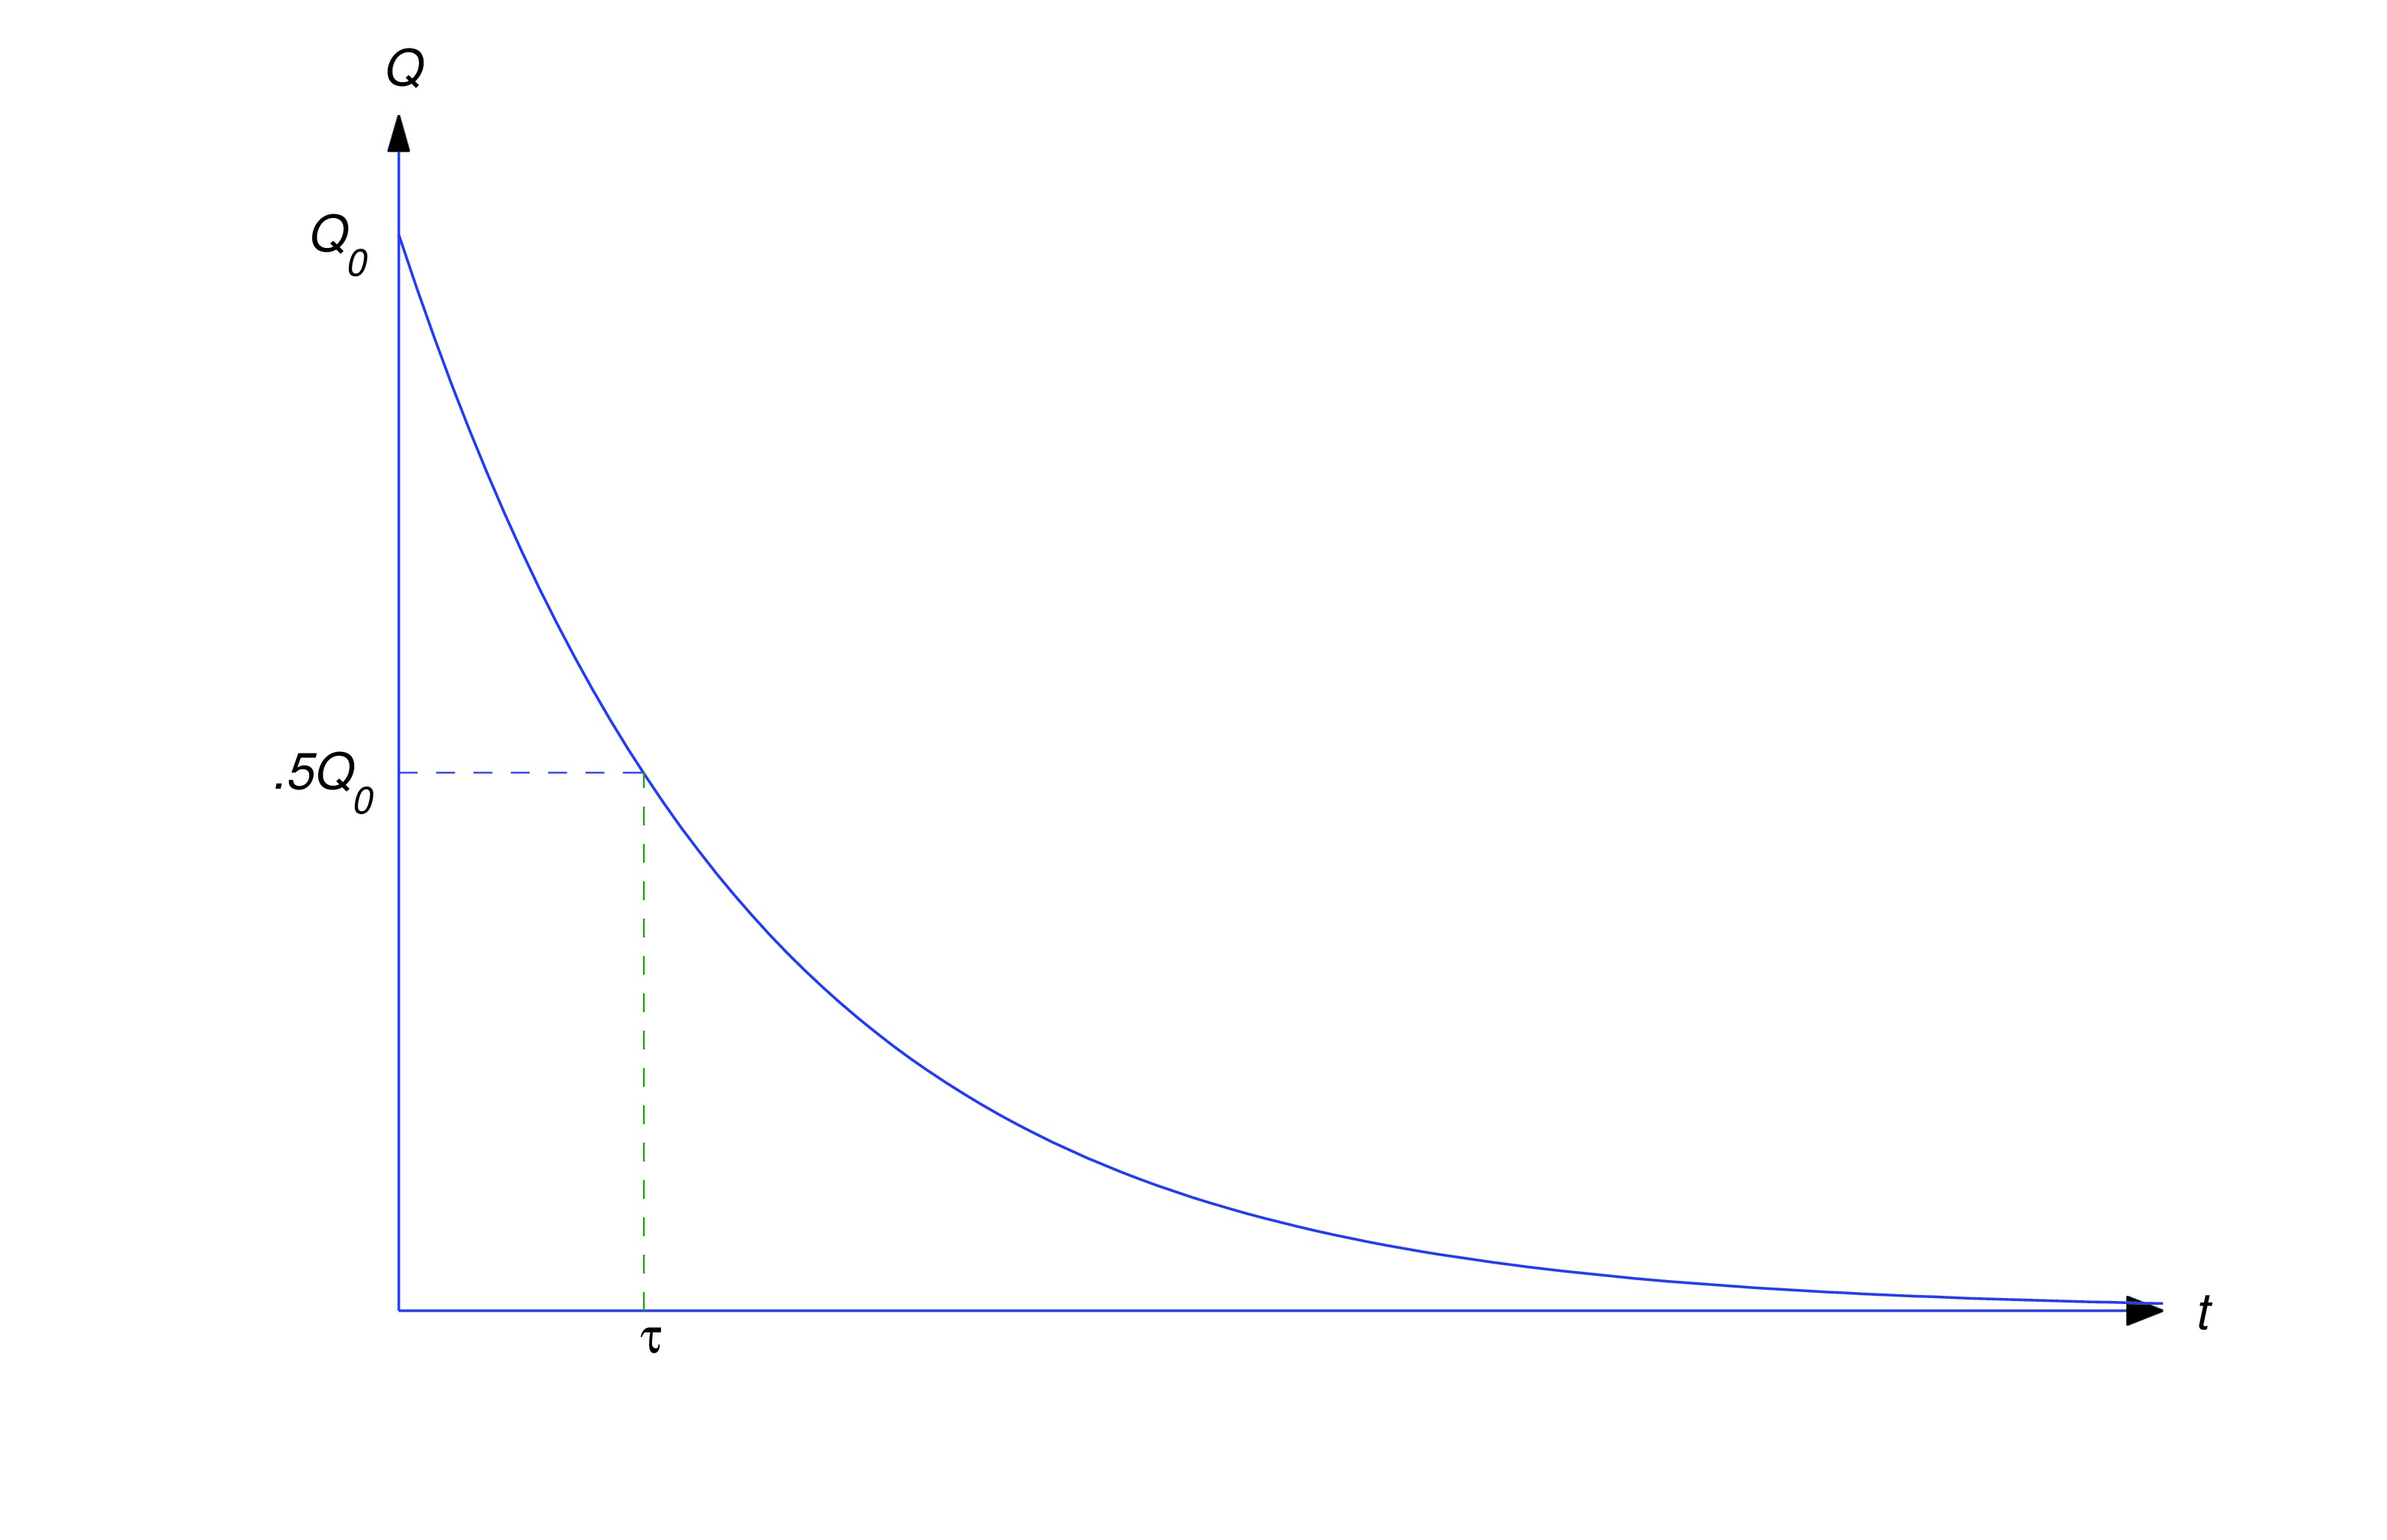
\includegraphics[height=1.5in]{fig040102.jpg} 
\end{image}

% \begin{figure}[tbp]
%   \centering
%   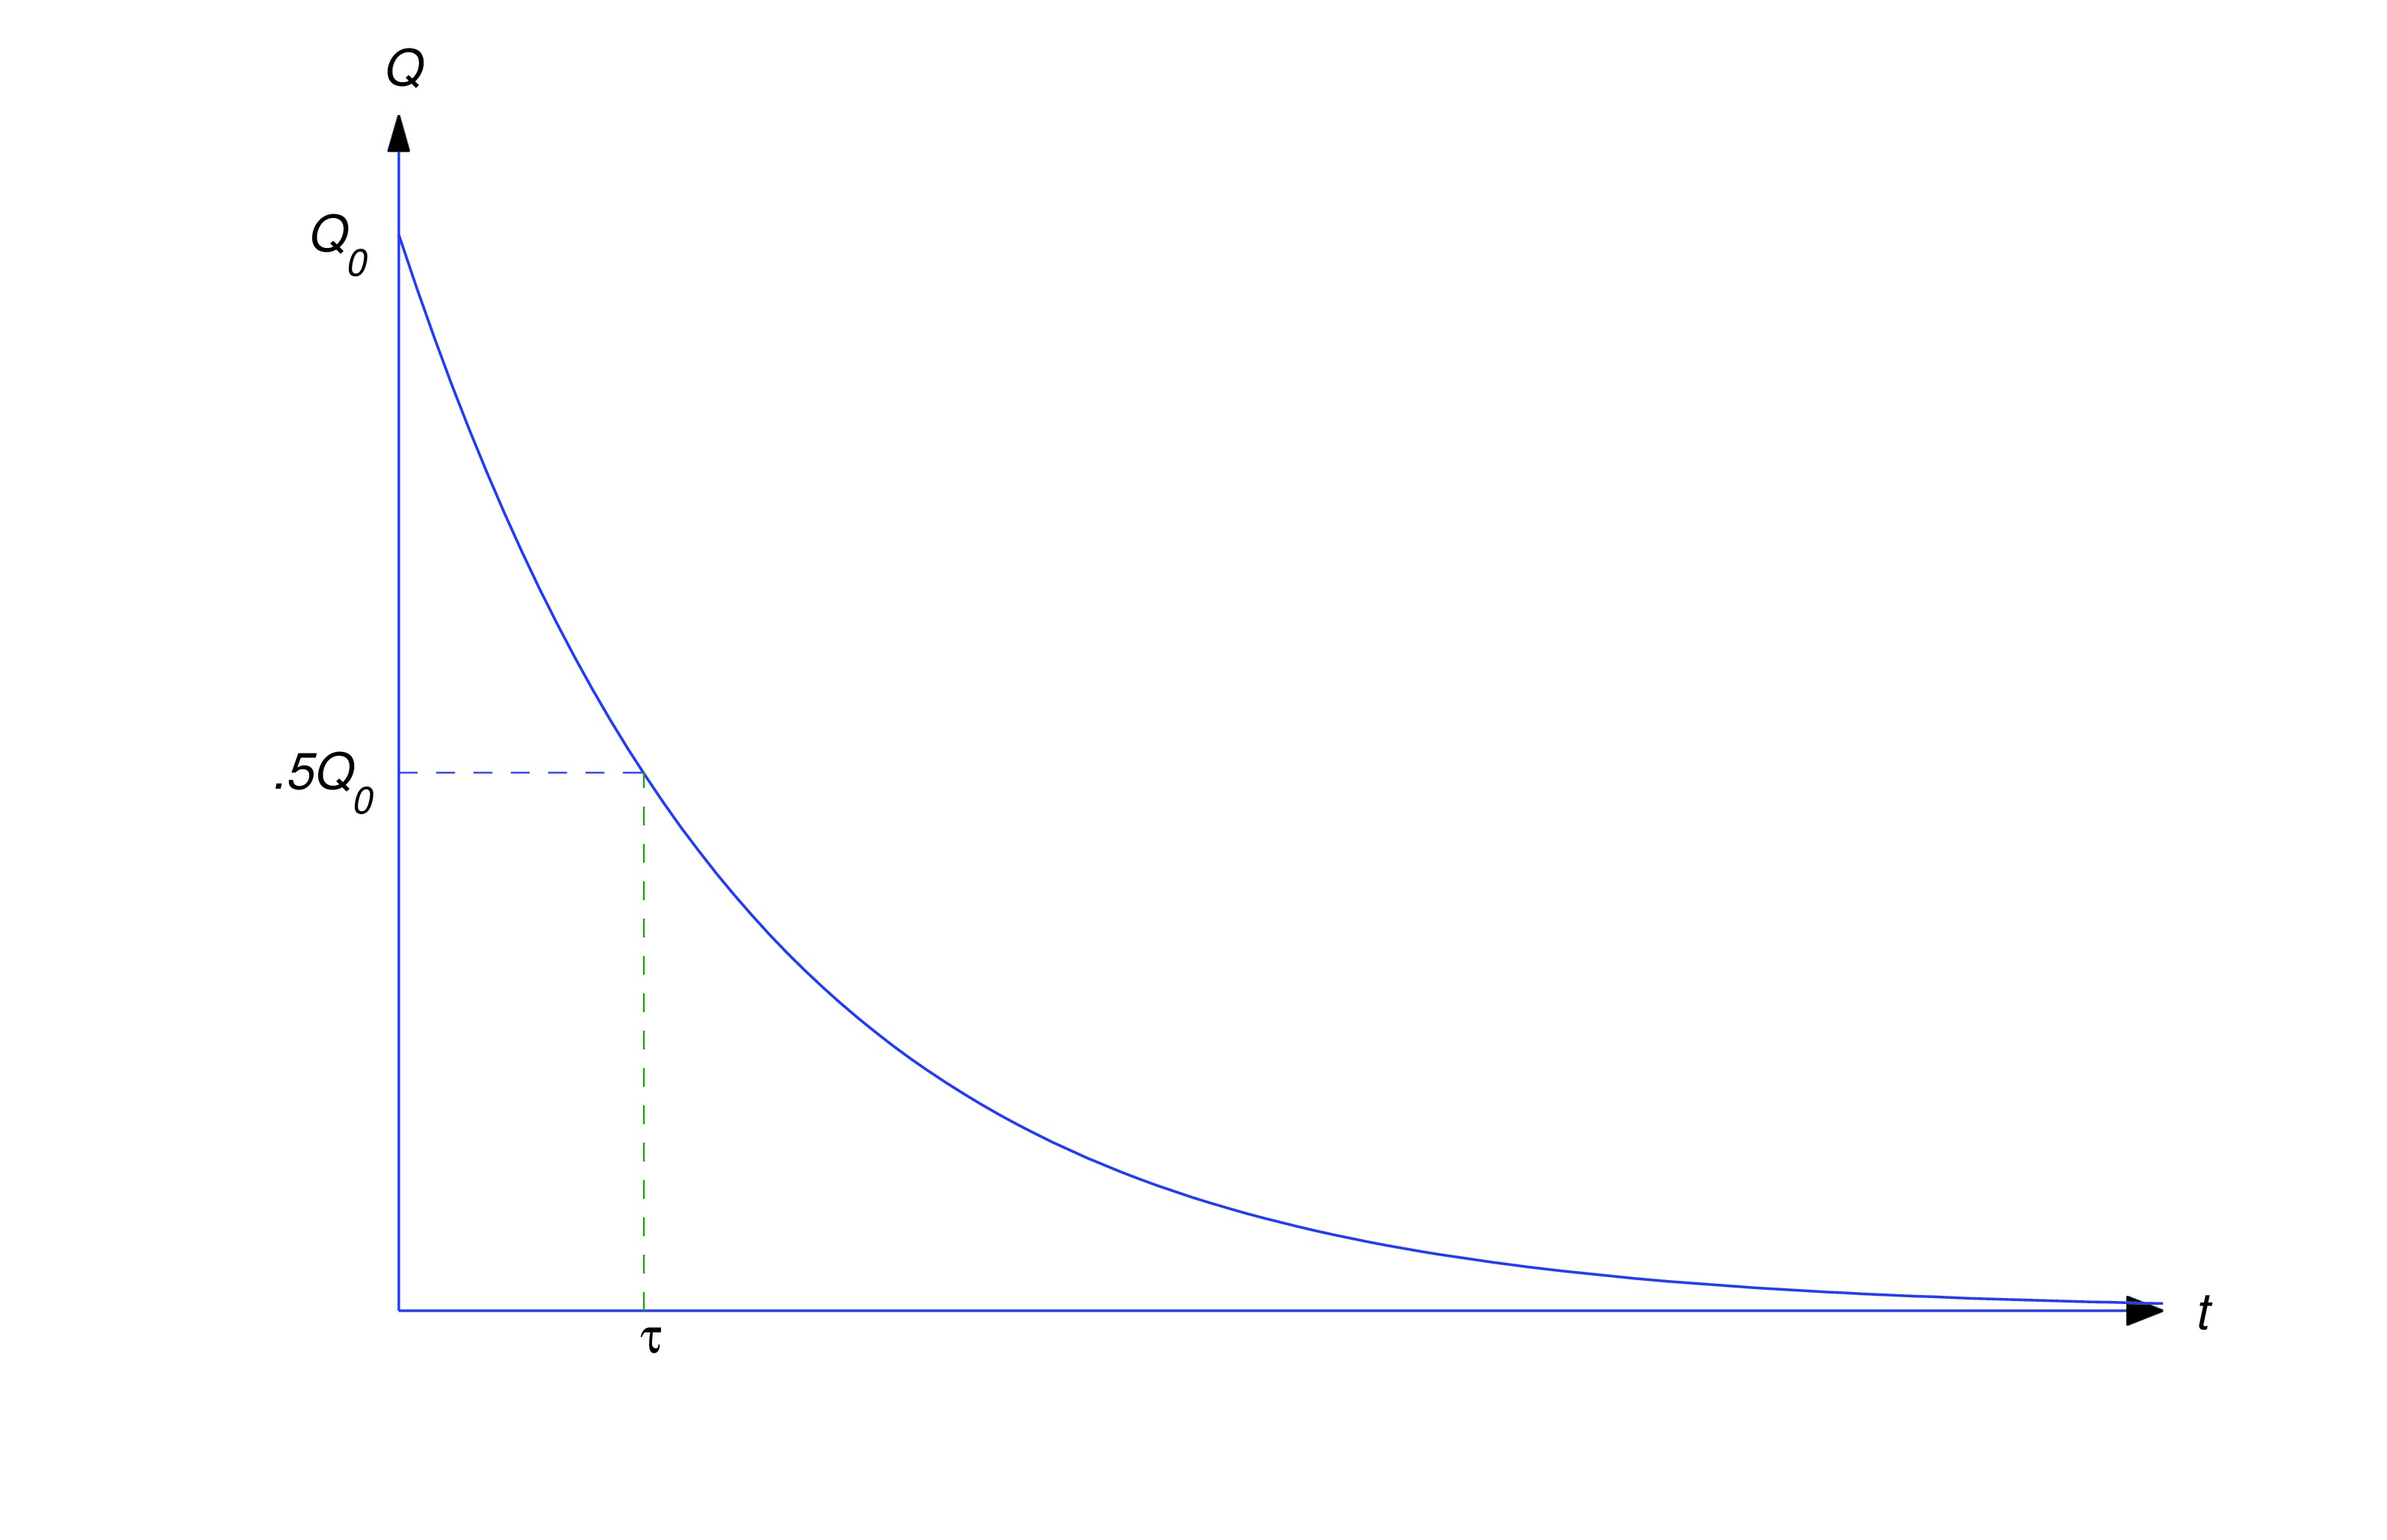
\includegraphics[bb=-78 148 689 643,width=5.67in,height=3.66in,keepaspectratio]{fig040102}
% \color{blue}
% \caption{Half-life of a radioactive substance}
%   \label{figure:4.1.2}
% \end{figure}

\begin{example}\label{example:4.1.1}
A  radioactive substance has a half-life of 1620 years.
\begin{enumerate}
\item \label{item:4.1.1a}%(a)
If its mass is now 4 g (grams), how much will be left 810 years
from now?
\item \label{item:4.1.1b}% (b)
Find the time $t_1$ when 1.5 g of the substance remain.
\end{enumerate}
\begin{explanation}
\ref{item:4.1.1a}  From \eqref{eq:4.1.3} with $t_0=0$ and
$Q_0=4$,
\begin{equation} \label{eq:4.1.6}
Q=4e^{-kt},
\end{equation}
 where we determine $k$ from \eqref{eq:4.1.5}, with $\tau$=
1620 years:
$$
k=\frac{\ln2}{\tau}=\frac{\ln2}{1620}.
$$
 Substituting this in \eqref{eq:4.1.6} yields
\begin{equation} \label{eq:4.1.7}
Q=4e^{-(t\ln2)/1620}.
\end{equation}
 Therefore the mass left after 810 years will be
$$\begin{array}{rl}
Q(810) &=4e^{-(810\ln2)/1620}=4e^{-(\ln2)/2} \\
&=2\sqrt{2} \mbox{ g}.
\end{array}$$

\ref{item:4.1.1b}
 Setting $t=t_1$  in \eqref{eq:4.1.7} and requiring that
$Q(t_1)=1.5$ yields
$$
\frac{3}{2}=4e^{(-t_1\ln2)/1620}.
$$
Dividing by 4 and taking logarithms yields
$$
\ln\frac{3}{8}=-\frac{t_1\ln2}{1620}.
$$
Since $\ln3/8=-\ln8/3$,
$$
t_1=1620\frac{\ln8/3}{\ln2}\approx  2292.4\quad\mbox{ years}.
$$
\end{explanation}
\end{example}

\subsection*{Interest Compounded Continuously}

Suppose we deposit an amount of money $Q_0$  in an
interest-bearing account and make no further deposits or withdrawals
for $t$ years, during which the account bears interest at a constant
annual rate $r$. To calculate the value of the account at the
end of $t$ years, we need one more piece of information: how the
interest is added to the account, or---as the bankers say---how it
is \textit{compounded}. If the interest is compounded annually,  the
value of the account is multiplied by $1+r$ at the end of each year.
This means that after $t$ years the value of the account is
$$
Q(t)=Q_0(1+r)^t.
$$
If interest is compounded semiannually,  the
value of the account is multiplied by $(1+r/2)$ every 6 months.
Since this occurs twice annually, the value of the account after $t$
years is
$$
Q(t)=Q_0\left(1+\frac{r}{2}\right)^{2t}.
$$
In general, if interest is compounded $n$ times per year, the value of
the account is multiplied $n$ times per year by $(1+r/n)$;  therefore,
the value of the account
after $t$ years is
\begin{equation} \label{eq:4.1.8}
Q(t)=Q_0\left(1+\frac{r}{n}\right)^{nt}.
\end{equation}
Thus, increasing the  frequency of  compounding increases the value of the
account after a fixed period of time. The table below shows the
effect
of increasing the number of compoundings over $t=5$ years on an initial
deposit of $Q_0=100$ (dollars), at an annual interest rate of 6\%.


$$\begin{array}{|c|c|}\hline
n & \$100 \left(1+\frac{.06}{n}\right)^{5n}\\
\text{(number of compoundings} &   \text{(value in dollars}\\
\text{per year)} &\text{after 5 years)}\\
\hline
1 & \$133.82 \\
2 & \$134.39 \\
4 & \$134.68 \\
8 & \$134.83 \\
364 & \$134.98 \\\hline
\end{array}$$


You can see from the table above that the value of the account after 5 years is an increasing function of $n$. Now suppose the maximum
allowable rate of interest on savings accounts is restricted by law,
but the number of times a bank can compound in a given time interval isn't;  %time intervals between successive compoundings isn't ; 
then competing banks can attract savers by compounding often. The ultimate step in this direction is to \textit{compound continuously}, by which we mean that $n\rightarrow\infty$ in \eqref{eq:4.1.8}. Since we know from calculus
that
$$
\lim_{n\rightarrow\infty} \left(1+{r}{n}\right)^n=e^r,
$$
 this yields
$$\begin{array}{rl}
Q(t) & =\lim_{n\rightarrow\infty} Q_0\left(1+\frac{r}{n}\right)^{nt}=Q_0 \left[
\lim_{n\rightarrow\infty} \left(1+\frac{r}{n}\right)^n\right]^t \\
&=Q_0e^{rt}.
\end{array}$$
Observe that $Q=Q_0e^{rt}$ is the solution of the initial value problem
$$
Q'=rQ, \quad Q(0)=Q_0;
$$
 that is, with continuous compounding the value of the account
grows exponentially.

\begin{example}\label{example:4.1.2}
If \$150 is deposited in a bank that pays
$5\frac{1}{2}$\% annual
interest compounded continuously,  the value of the account after
$t$ years is
$$
Q(t)=150e^{.055t}
$$
dollars. (Note that it's necessary to write the interest rate as a
decimal;   thus, $r=.055$.) Therefore, after $t=10$ years the value
of the account is
$$
Q(10)=150e^{.55} \approx \$259.99.
$$
\end{example}

\begin{example}\label{example:4.1.3}
We wish to accumulate \$10,000 in 10 years by making a single deposit
in a savings account bearing $5\frac{1}{2}$\% annual interest
compounded continuously. How much must we deposit in the account?


\begin{explanation}  
The value of the account at time $t$ is
\begin{equation} \label{eq:4.1.9}
Q(t)=Q_0e^{.055t}.
\end{equation}
Since we want $Q(10)$ to be \$10,000, the initial deposit $Q_0$ must
satisfy the equation
\begin{equation} \label{eq:4.1.10}
10000=Q_0e^{.55},
\end{equation}
 obtained by setting $t=10$ and $Q(10)=10000$ in
\eqref{eq:4.1.9}.  Solving \eqref{eq:4.1.10} for $Q_0$ yields
$$
Q_0=10000e^{-.55} \approx \$5769.50.
$$
\end{explanation}
\end{example}

\subsection*{Mixed Growth and Decay}

\begin{example}\label{example:4.1.4}
A radioactive substance with decay constant $k$ is produced at a
constant rate of $a$ units of mass per unit time.
\begin{enumerate}
\item \label{item:4.1.4a}%(a)
Assuming that $Q(0)=Q_0$, find the mass $Q(t)$ of the
substance present at time~$t$.

\item \label{item:4.1.4b}%(b)
Find $\lim_{t\rightarrow\infty} Q(t)$.
\end{enumerate}
\begin{explanation}
\ref{item:4.1.4a}  Here
$$
Q'=\mbox{ rate of increase of } Q - \mbox{ rate of decrease
of } Q.
$$
The rate of increase is the constant $a$. Since $Q$ is radioactive
with decay constant $k$, the rate of decrease is $kQ$. Therefore
$$
Q'=a-kQ.
$$
This is a linear first order differential equation. Rewriting it and
imposing the initial condition shows that $Q$ is the solution of the
initial value problem
\begin{equation}  \label{eq:4.1.11}
Q'+kQ=a, \quad Q(0)=Q_0.
\end{equation}
% Since
% $e^{-kt}$ is a solution of the complementary equation, the solutions
% of \eqref{eq:4.1.11} are of the form $Q=ue^{-kt}$, where $u'e^{-kt}=a$, so
% $u'=ae^{kt}$. Hence,
% $$
% u={a\over k}e^{kt}+c
% $$
% and
% $$
% Q=ue^{-kt}={a\over k}+ce^{-kt}.
% $$
Proceeding as we did in Module \href{https://ximera.osu.edu/ode/main/linearFirstOrderDiffEq/linearFirstOrderDiffEq}{linearFirstOrderDiffEq}, we compute $$Q=ue^{-kt}=\frac{a}{k}+ce^{-kt}.$$
 Since $Q(0)=Q_0$, setting $t=0$ here yields
$$Q_0=\frac{a}{k}+c  \quad\mbox{or}\quad c=Q_0-\frac{a}{k}.$$
 Therefore
\begin{equation} \label{eq:4.1.12}
Q=\frac{a}{k}+\left(Q_0-\frac{a}{k}\right)e^{-kt}.
\end{equation}

\ref{item:4.1.4b}
Since $k > 0$,  $\lim_{t\rightarrow\infty} e^{-kt}=0$, so
from \eqref{eq:4.1.12}
$$
\lim_{t\rightarrow\infty} Q(t)=\frac{a}{k}.
$$
This limit depends only on $a$ and $k$, and not on $Q_0$.
We say that $a/k$ is the \textit{steady state} value of $Q$. From
\eqref{eq:4.1.12} we also see that $Q$ approaches its steady state value
from above if $Q_0 > a/k$, or from below if $Q_0 < a/k$. If $Q_0=a/k$,
then $Q$ remains constant (see figure below).
%(Figure \ref{figure:4.1.3}).

\begin{image}
 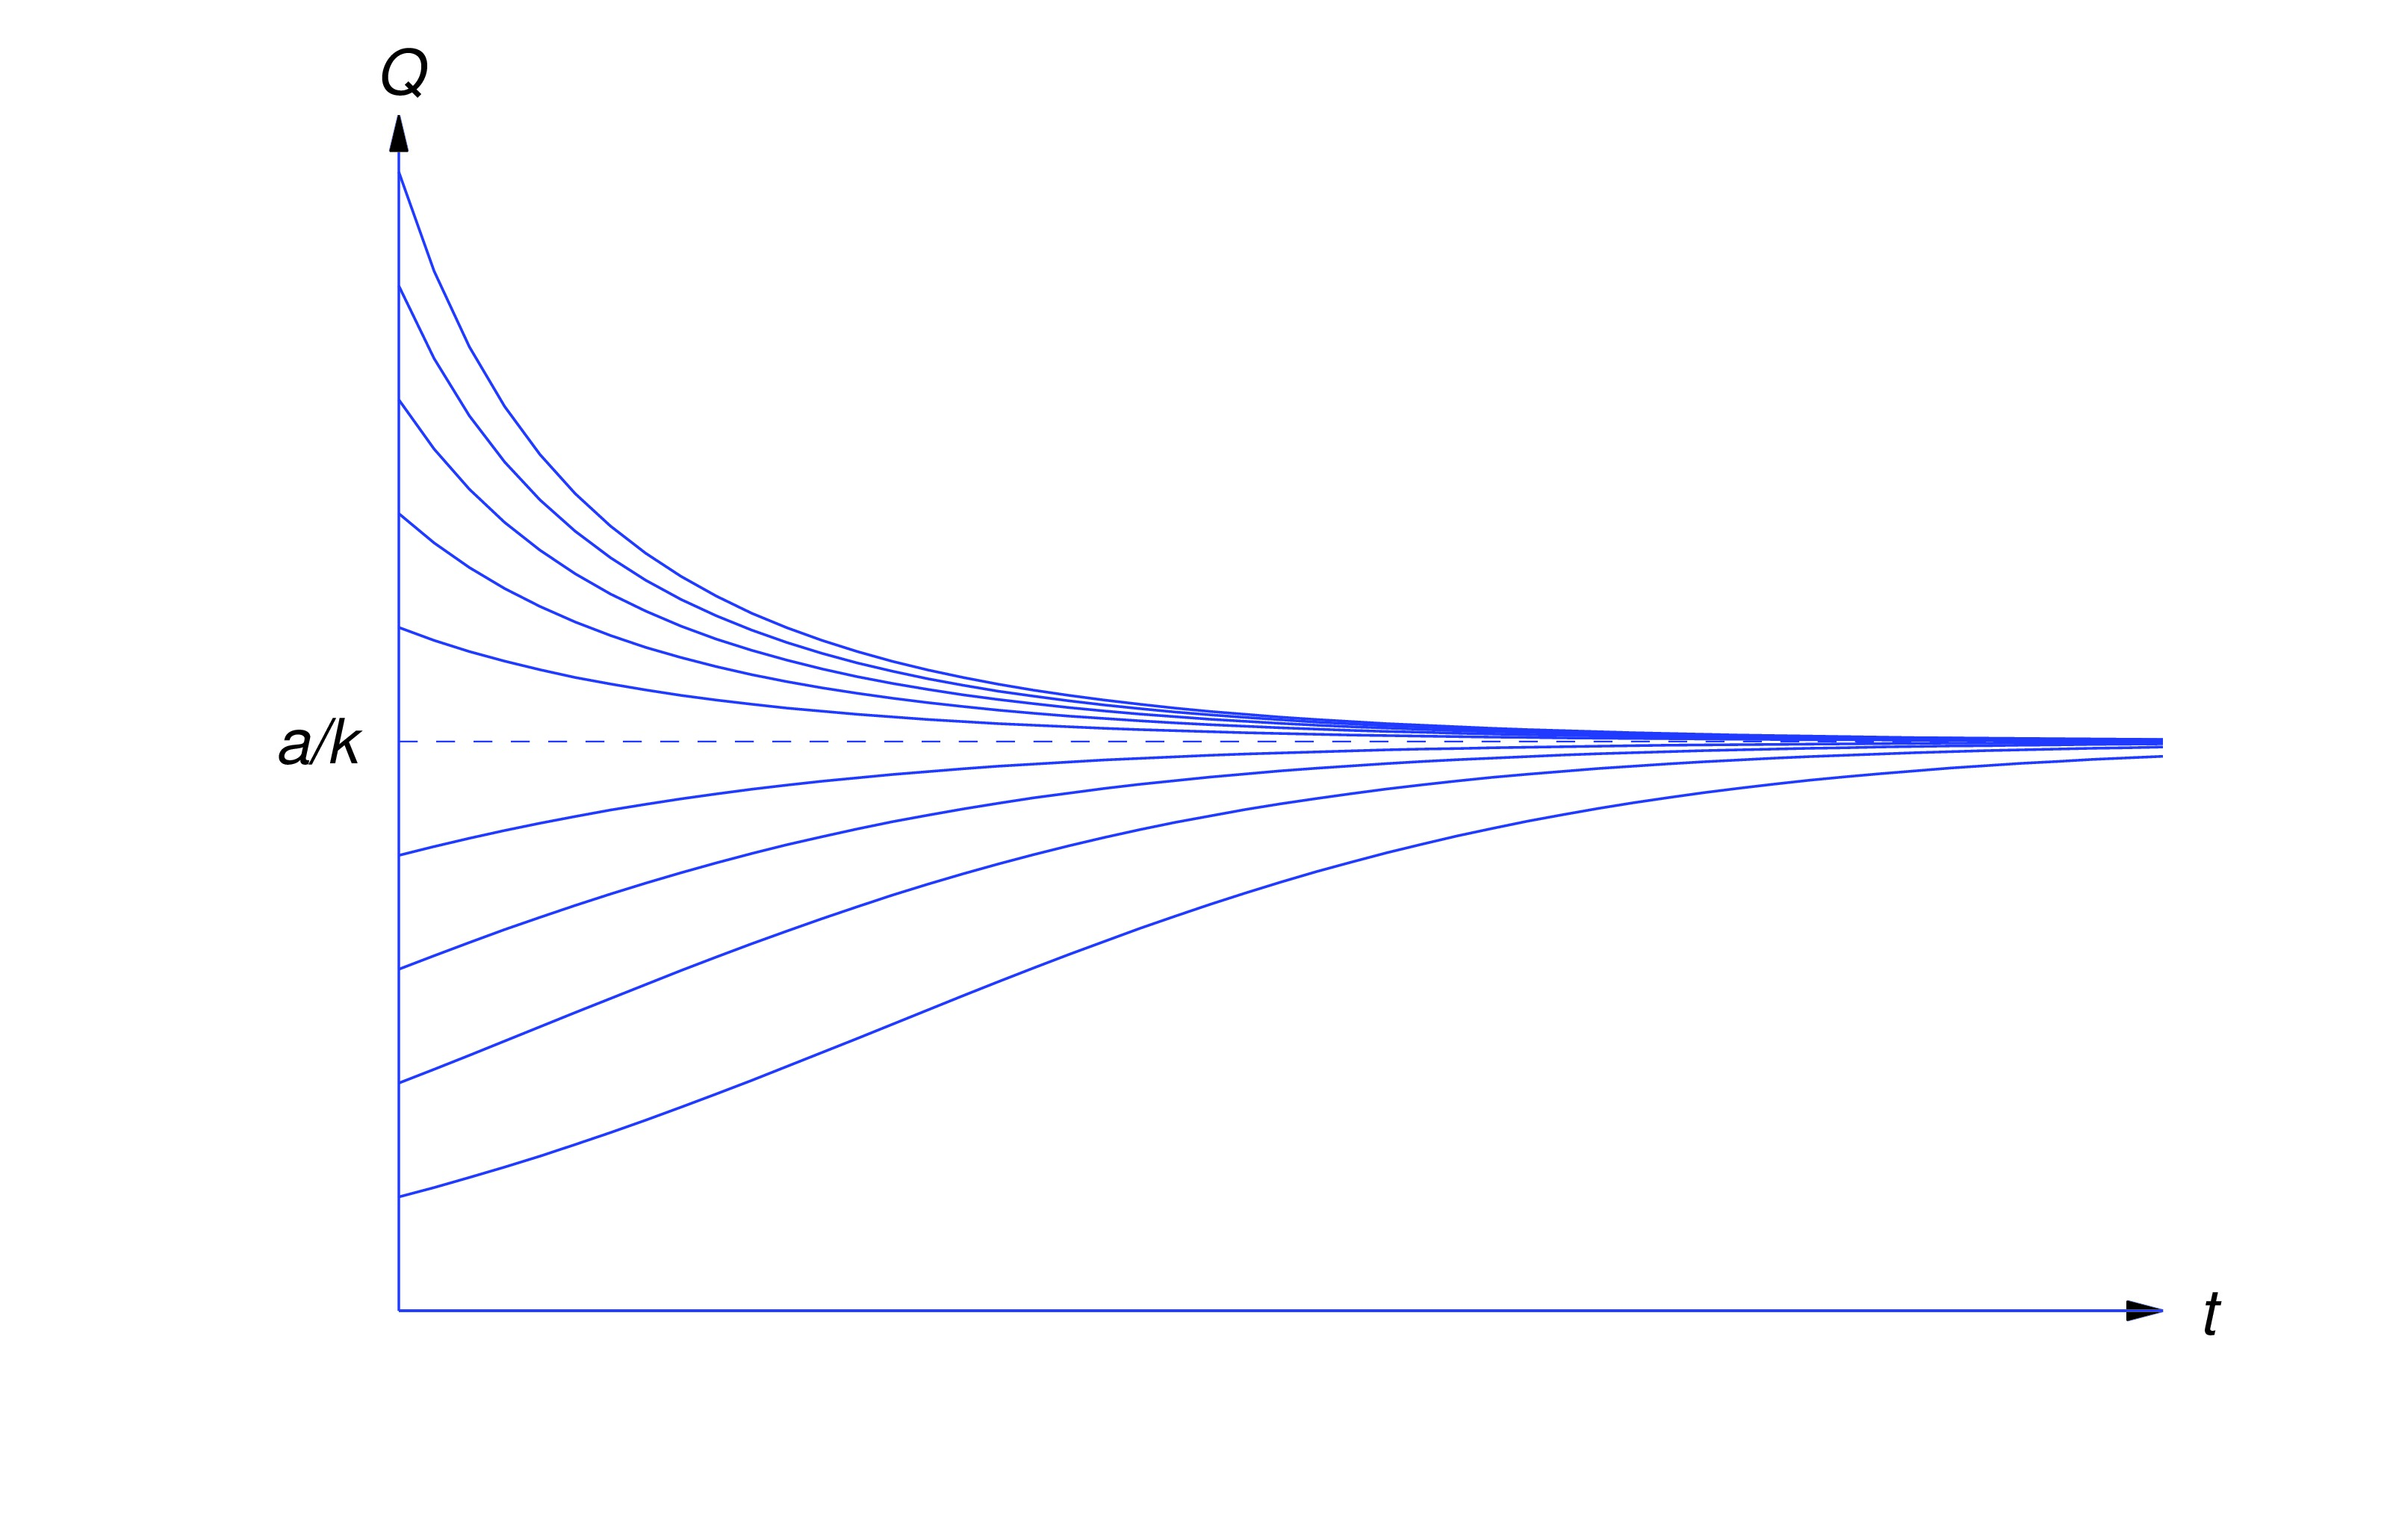
\includegraphics[height=1.5in]{fig040103.jpg} 
 \end{image}

\end{explanation}
\end{example}

% \begin{figure}[tbp]
%   \centering
%   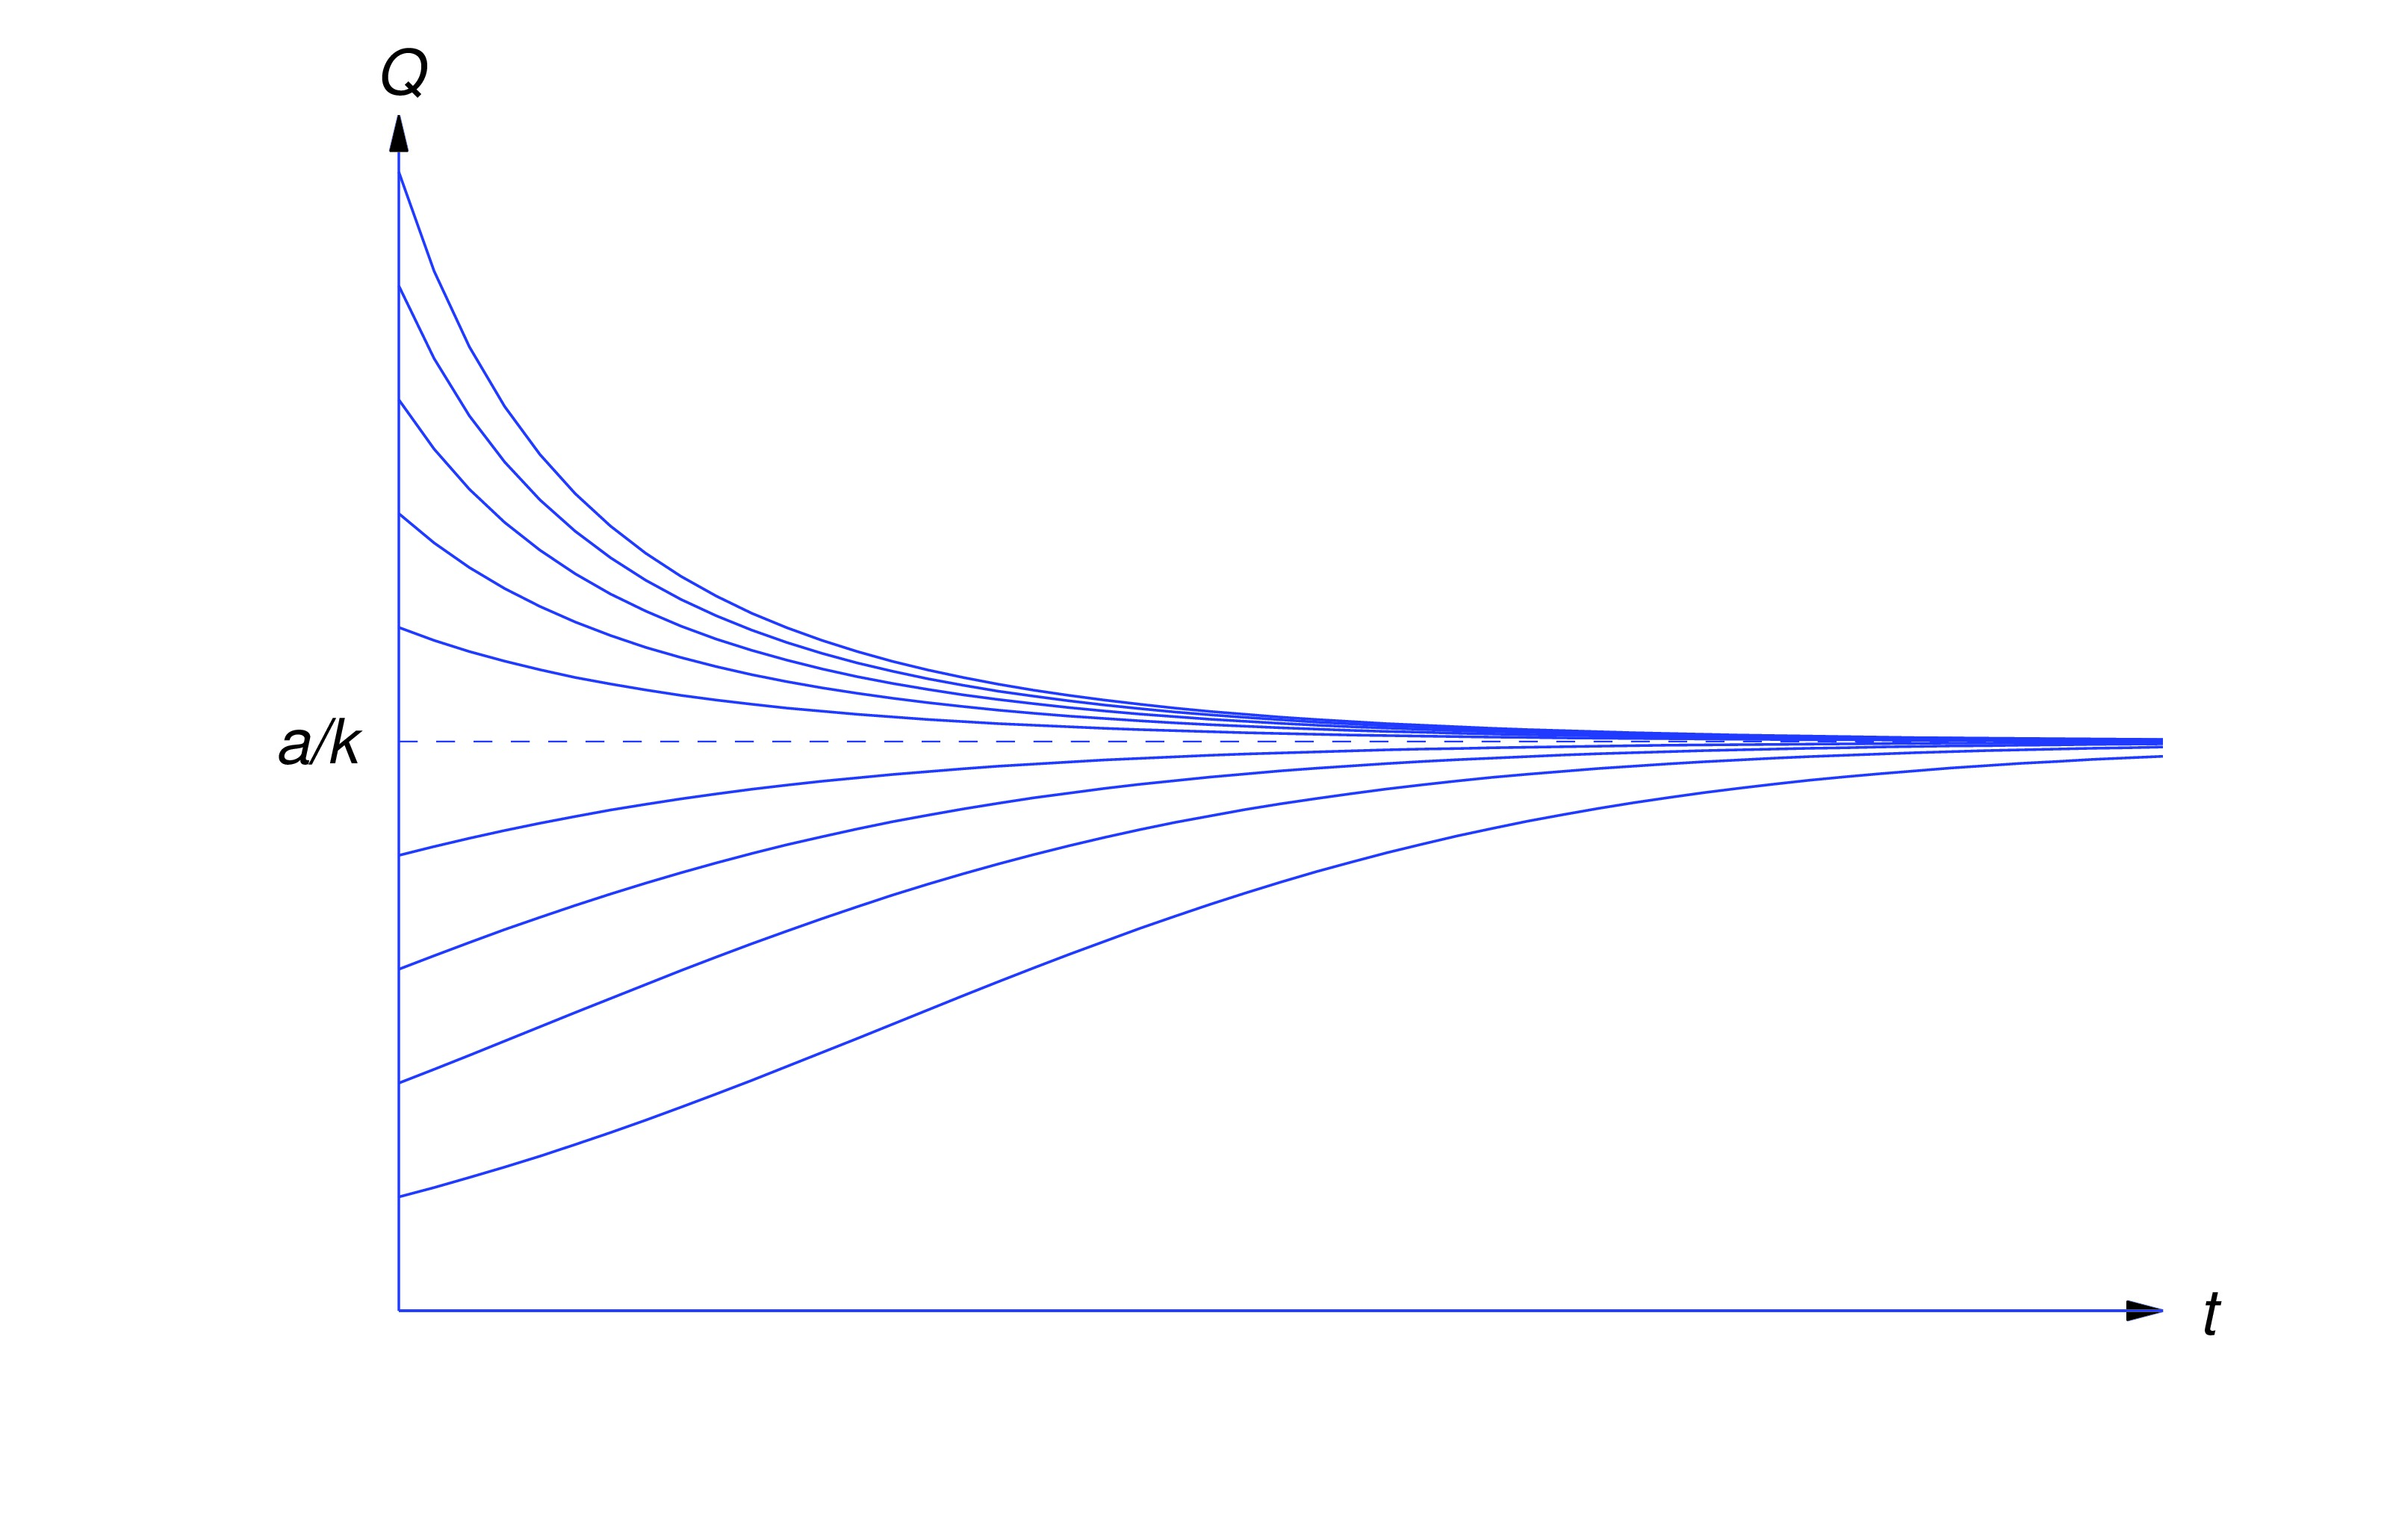
\includegraphics[bb=-78 148 689 643,width=5.67in,height=3.66in,keepaspectratio]{fig040103}
% \color{blue}
% \caption{$Q(t)$ approaches the steady state value
% $ {a\over k}$ as $t\rightarrow\infty$}
%   \label{figure:4.1.3}
% \end{figure}


\subsection*{Carbon Dating}

The fact that $Q$ approaches a steady state value in the
situation discussed in Example 4 underlies the method of \textit{carbon dating}, devised by the American chemist and Nobel Prize Winner
\href{http://www.nobelprize.org/nobel_prizes/chemistry/laureates/1960/libby-lecture.pdf}{W.S. Libby}.

Carbon 12 is stable, but carbon-14, which is produced by cosmic
bombardment of nitrogen in the upper atmosphere, is radioactive with a
half-life of about 5570 years. Libby assumed that the
quantity
of carbon-12 in the atmosphere has been constant throughout time, and
that the quantity of radioactive carbon-14 achieved its steady state
value long ago as a result of its creation and decomposition over
millions of years. These assumptions led Libby to conclude that the
ratio of carbon-14 to carbon-12 has been nearly constant for a long
time. This constant, which we denote by $R$, has been determined
experimentally.

Living cells absorb both carbon-12 and carbon-14 in the proportion in
which they are present in the environment. Therefore the ratio of
carbon-14 to carbon-12 in a living cell is always $R$. However, when
the cell dies it ceases to absorb carbon, and the ratio of carbon-14
to carbon-12 decreases exponentially as the radioactive carbon-14
decays. This is the basis for the method of carbon dating, as
illustrated in the next example.

\begin{example}\label{example:4.1.5}
An archaeologist investigating the site of an ancient village finds a
burial ground where the amount of carbon-14 present in individual
remains is between 42 and 44\% of the amount present in live
individuals. Estimate the age of the village and the length of time
for which it survived.
\begin{explanation}
Let $Q=Q(t)$ be the quantity of carbon-14 in an individual
set of remains $t$ years after death, and let $Q_0$ be the quantity
that would be present in  live individuals.
Since carbon-14 decays exponentially with half-life 5570 years, its
decay constant is
$$
k=\frac{\ln2}{5570}.
$$
 Therefore
$$
Q=Q_0e^{-t(\ln2)/5570}
$$
 if we choose our time scale so that $t_0=0$ is the
time of death.  If we know the present value of $Q$  we
can solve this equation for $t$, the number of years since
death occurred.  This yields
$$
t=-5570 \frac{\ln Q/Q_0}{\ln2}.
$$
It is given that $Q=.42Q_0$ in the remains of individuals who died
first. Therefore these deaths occurred about
$$
t_1=-5570 \frac{\ln .42}{\ln2} \approx 6971
$$
 years ago.  For the most recent deaths, $Q=.44
Q_0$; hence, these deaths occurred about
$$
t_2=-5570 \frac{\ln .44}{\ln2} \approx 6597
$$
 years ago.  Therefore it's reasonable to conclude
that the village was founded about 7000 years ago,
and lasted for about 400 years.
\end{explanation}
\end{example}

\subsection*{A Savings Program}

\begin{example}\label{example:4.1.6}
A person opens a savings account with an initial deposit of \$1000 and
subsequently deposits \$50 per week. Find the value $Q(t)$ of the
account at time $t > 0$, assuming that the bank pays 6\%
interest compounded continuously.
\begin{explanation}
Observe that $Q$ isn't  continuous, since there are 52
discrete deposits per year of \$50 each. To construct a mathematical
model for this problem in the form of a differential equation, we make
the simplifying assumption that the deposits are made continuously at
a rate of \$2600 per year. This is essential, since solutions of
differential equations are continuous functions. With this assumption,
$Q$ increases continuously at the rate
$$
Q'=2600+.06 Q
$$
and therefore $Q$ satisfies the differential equation
\begin{equation} \label{eq:4.1.13}
Q'-.06Q=2600.
\end{equation}
(Of course, we must recognize that the solution of this equation
is an approximation to the true value of $Q$ at any given time. We'll
discuss this further below.)  
% Since $e^{.06t}$ is a solution of the complementary equation, the solutions of \eqref{eq:4.1.13}  are of the
% form   $Q=ue^{.06t}$,  where $u'e^{.06t}=2600$. Hence,
% $u'=2600e^{-.06t}$,
% $$
% u=- {2600\over .06}e^{-.06t}+c
% $$
% and
Proceeding as we did in Module \href{https://ximera.osu.edu/ode/main/linearFirstOrderDiffEq/linearFirstOrderDiffEq}{linearFirstOrderDiffEq}, we compute
\begin{equation} \label{eq:4.1.14}
%Q=ue^{.06t}=-\frac{2600}{.06}+ce^{.06t}.
Q=-\frac{2600}{.06}+ce^{.06t}.
\end{equation}
 Setting $t=0$ and $Q=1000$ here yields
$$
c=1000+\frac{2600}{.06},
$$
and substituting this into \eqref{eq:4.1.14} yields
\begin{equation} \label{eq:4.1.15}
Q=1000e^{.06t}+\frac{2600}{.06}(e^{.06t}-1),%\tag15
\end{equation}
where the first term is the value due to the initial deposit and the
second is due to the subsequent weekly deposits.
\end{explanation}
\end{example}

Mathematical models must be tested for validity by comparing
predictions based on them with the actual outcome of experiments.
Example 6 is unusual in that we can compute the exact value of the
account at any specified time and compare it with the approximate
value predicted by \eqref{eq:4.1.15} %(See Exercise \ref{exer:4.1.21}.). 
The following table gives a comparison for a ten year period. Each exact answer corresponds to the time of the year-end deposit, and each year is assumed to have exactly 52 weeks.

$$
\begin{array}{c|c|c|c|c}
\text{Year} & \text{Approximate Value of } Q & \text{Exact Value} & \text{Error} & \text{Percentage
Error}\\
& \text{(Example~\ref{example:4.1.6})} & \text{of } P
& Q-P &
(Q-P)/P\\
\hline
  1 & \$ 3741.42 & \$ 3739.87 & \$ 1.55 &.0413 \% \\
  2 &   6652.36 &  6649.17 & 3.19 &.0479\\
  3 & 9743.30 &9738.37 &4.93 &.0506\\
  4 &  13,025.38 &  13,018.60 &6.78 & .0521\\
  5 &  16,510.41 &  16,501.66 & 8.75 &.0530 \\
  6 &  20,210.94 &  20,200.11 & 10.83 & .0536\\
  7 &  24,140.30 &  24,127.25 & 13.05 &.0541 \\
  8 &  28,312.63 &  28,297.23 & 15.40 &.0544 \\
  9 &  32,742.97 &  32,725.07 & 17.90 & .0547 \\
 10 &  37,447.27 &  37,426.72 & 20.55 & .0549 
 \end{array}
$$


\section*{Text Source}
Trench, William F., "Elementary Differential Equations" (2013). Faculty Authored and Edited Books \& CDs. 8. (CC-BY-NC-SA)

\href{https://digitalcommons.trinity.edu/mono/8/}{https://digitalcommons.trinity.edu/mono/8/}


\end{document}